% Document the final deployment of your application.
% • Visualize the structure of the deployment (the entities and their connections).
% • The diagram should illustrate the data flow for incoming requests.
% • Include all resources that you have deployed in the cluster and their connections (not just the ones that are relevant for serving requests).
% • Clarify the visualization through a concise elaboration.

% Insufficient -> The deployment documentation is incomprehensible or incomplete.
% Sufficient -> The deployment documentation is limited to the structure of the deployment (the entities and their connections) or the data flow for incoming requests. The documentation visualizes the deployment and connects the text.
% Good -> The deployment documentation describes both the structure of the deployment (the entities and their connections) and the data flow for incoming requests.
% Very Good -> The deployment documentation includes all deployed resource types and relations.
% Excellent -> The deployment documentation is visually appealing and clear. It is easy for a new team member to understand and to start contributing to the described system.

% Interesting visualization tool:
% https://diagrams.mingrammer.com/docs/getting-started/examples

\section{Deployment}
We host our application on a set of virtual machine (VM) nodes. This is achieved using {\color{blue} \href{https://www.vagrantup.com/}{Vagrant}} and {\color{blue} \href{https://www.ansible.com/}{Ansible}}. Vagrant is a tool used to create and manage VM environments in a single workflow. Then, Ansible is an automation tool for provisioning, configuring, and managing the VMs.

The actual provisioning and deployment is done using {{\color{blue} \href{https://kubernetes.io/}{Kubernetes}}}.
Our deployment consists of multiple services and deployments managed within a Kubernetes cluster, utilizing {\color{blue} \href{https://istio.io/}{Istio}} for advanced traffic management. See figure {\color{red} \ref{fig:k8s_istio}}. The core components include frontend and backend services, along with a model service.

The app-frontend service has two versions of deployments (app-frontend-v1 and app-frontend-v2), each running with one replica. The app-service and model-service are also deployed with a single replica each, exposing ports 3000 and 5000, respectively.

We use Istio to manage the ingress traffic through the app-gateway, which is configured to listen on port 80 for HTTP traffic. The app-virtualservice directs traffic to different services based on the URI path. Requests with the prefix '/app' are routed to the app-frontend service, with 80\% of the traffic directed to version 1 and 20\% to version 2. Requests to '/api' are routed to the app-service on port 3000, and requests to '/model' are routed to the model-service on port 5000. Additionally, installed using {\color{blue} \href{https://helm.sh/}{Helm}}, we use monitoring tools like {\color{blue}\href{https://prometheus.io/docs/introduction/overview/}{Prometheus}} and {\color{blue} \href{https://duckduckgo.com/?q=grafana&ia=web}{Grafana}} to collect and monitor metrics. The corresponding '/metrics' and '/grafana' paths are directed to   services for monitoring and visualization purposes. 

This setup allows for robust service management, version control, and traffic routing, ensuring high availability and scalability of our application.


\begin{figure}[h]
    \centering
    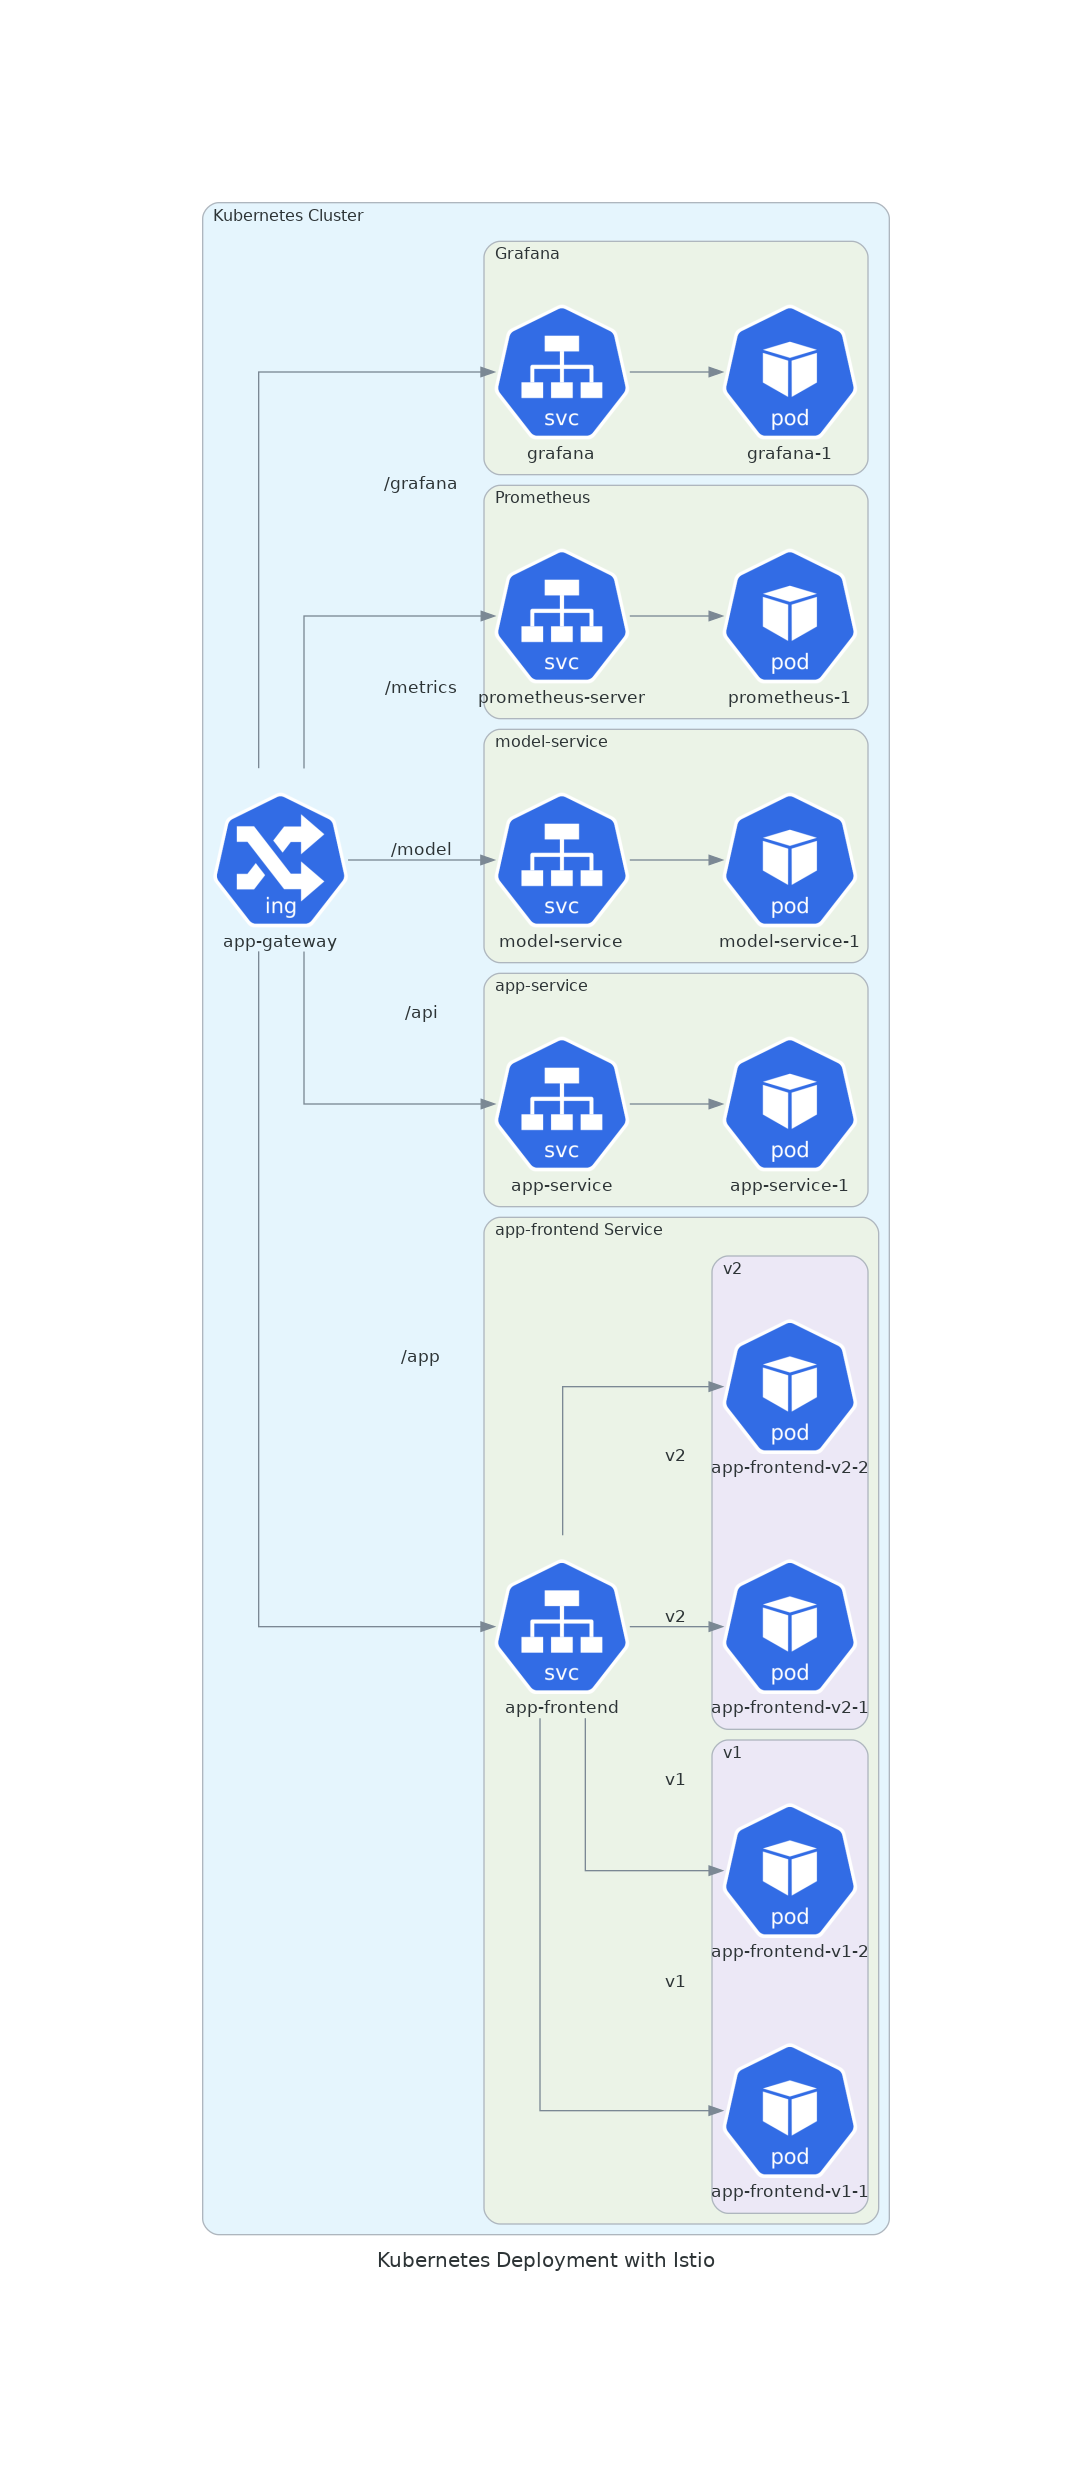
\includegraphics[width=\linewidth]{kubernetes_deployment_with_istio.png}
    \caption{Diagram of Kubernetes Deployment with Istio Gateway and Virtual Services}
    \label{fig:k8s_istio}
\end{figure}


